\documentclass[aspectratio=169,12pt]{beamer}
% Build from the repository root: make lecture-07-slides
\usepackage[T1]{fontenc}
\usepackage{lmodern}
\usepackage{amsmath,amssymb,booktabs,array}
\usepackage{pgfplots}
\pgfplotsset{compat=1.18}
\usefonttheme{professionalfonts}
\definecolor{Ink}{HTML}{16324F}
\definecolor{Blue}{HTML}{1F4E79}
\definecolor{Orange}{HTML}{C46A13}
\definecolor{Teal}{HTML}{007D80}
\setbeamercolor{normal text}{fg=Ink,bg=white}
\setbeamercolor{frametitle}{fg=Ink}
\setbeamercolor{structure}{fg=Blue}
\setbeamerfont{frametitle}{size=\large,series=\bfseries}
\setbeamersize{text margin left=8mm,text margin right=8mm}
\setbeamertemplate{navigation symbols}{}
\setbeamertemplate{headline}{}
\setbeamertemplate{footline}{}
\addtobeamertemplate{footline}{}{\vspace*{3mm}}
\setbeamertemplate{frametitle}{\vspace{3mm}\insertframetitle\par\vspace{1mm}}
\newcommand{\slidespacing}{%
  \setlength{\parskip}{0.2em}%
  \setlength{\abovedisplayskip}{0.3em}%
  \setlength{\belowdisplayskip}{0.3em}%
  \setlength{\abovedisplayshortskip}{0.1em}%
  \setlength{\belowdisplayshortskip}{0.2em}}
\newcommand{\Prob}{\mathbb P}
\newcommand{\Expect}{\mathbb E}
\DeclareMathOperator{\Var}{Var}
\DeclareMathOperator{\Cov}{Cov}
\newcommand{\KL}{D_{\mathrm{KL}}}
\newcommand{\CE}{\operatorname{CE}}
\newcommand{\plotcaption}[1]{\par\smallskip{\small #1\par}}
\setbeamertemplate{blocks}[default]
\setbeamerfont{block title}{size=\normalsize,series=\bfseries}
\setbeamerfont{block body}{size=\normalsize}
\newenvironment{coursebox}[2]{%
  \begingroup
  \setbeamercolor{block title}{fg=#1,bg=#1!13!white}
  \setbeamercolor{block body}{fg=Ink,bg=#1!4!white}
  \begin{block}{#2}
  \setlength{\parskip}{0.1em}
  \setlength{\abovedisplayskip}{0.3em}
  \setlength{\belowdisplayskip}{0.3em}
  \setlength{\abovedisplayshortskip}{0.1em}
  \setlength{\belowdisplayshortskip}{0.1em}
}{\end{block}\endgroup}
\newenvironment{definitionbox}[1]
  {\begin{coursebox}{Blue}{Definition: #1}}{\end{coursebox}}
\newenvironment{resultbox}[1]
  {\begin{coursebox}{Teal}{Result: #1}}{\end{coursebox}}
\newcommand{\InfoDataPath}{../../figures/data}
\newcommand{\InfoPlotWidth}{12cm}
\newcommand{\InfoPlotHeight}{3.5cm}
% Shared scientific charts for the notes and Lecture 7 slides.
\providecommand{\InfoDataPath}{figures/data}
\providecommand{\InfoPlotWidth}{11.8cm}
\providecommand{\InfoPlotHeight}{4.4cm}
\definecolor{InfoBlue}{HTML}{1F4E79}
\definecolor{InfoOrange}{HTML}{C46A13}
\definecolor{InfoTeal}{HTML}{007D80}
\definecolor{InfoMuted}{HTML}{526477}
\pgfplotsset{info axis/.style={
  scale only axis,width=\InfoPlotWidth,height=\InfoPlotHeight,
  axis lines=left,enlargelimits=false,
  grid=major,grid style={black!9},
  tick label style={font=\footnotesize},label style={font=\footnotesize},
  /pgf/number format/.cd,fixed,precision=2,/pgfplots/.cd,
  legend style={draw=none,fill=none,font=\footnotesize,
    at={(0.5,1.04)},anchor=south,legend columns=-1,column sep=0.7em},
  every axis plot/.append style={no marks,line width=1.15pt},
}}

\newcommand{\InfoEntropyPlot}{%
\begin{tikzpicture}\begin{axis}[info axis,
  xmin=0,xmax=1,ymin=0,ymax=0.74,
  xlabel={Success probability $p$},ylabel={Entropy $H(P_p)$, nats},
  xtick={0,0.2,0.5,0.8,1},ytick={0,0.2,0.4,0.693147},
  yticklabels={$0$,$0.2$,$0.4$,$\log 2$}]
  \addplot[InfoBlue] table[x=p,y=entropy] {\InfoDataPath/ch7-entropy.dat};
  \addplot[InfoOrange,only marks,mark=*,mark size=2pt]
    coordinates {(0.5,0.69314718056) (0.8,0.500402423538)};
\end{axis}\end{tikzpicture}%
}

\newcommand{\InfoCrossEntropyPlot}{%
\begin{tikzpicture}\begin{axis}[info axis,
  xmin=0.02,xmax=0.98,ymin=0,ymax=3.3,
  xlabel={Predicted success probability $q$},ylabel={Expected loss, nats},
  xtick={0.02,0.2,0.5,0.8,0.98},ytick={0,0.5,1,2,3},
  scaled ticks=false]
  \addplot[InfoBlue] table[x=q,y=ce] {\InfoDataPath/ch7-cross-entropy.dat};
  \addlegendentry{$\operatorname{CE}(P,Q)$}
  \addplot[InfoOrange,densely dotted] table[x=q,y=entropy] {\InfoDataPath/ch7-cross-entropy.dat};
  \addlegendentry{$H(P)$}
  \addplot[InfoTeal,dashed] table[x=q,y=kl] {\InfoDataPath/ch7-cross-entropy.dat};
  \addlegendentry{$D_{\mathrm{KL}}(P\Vert Q)$}
  \addplot[InfoMuted,densely dotted,forget plot]
    coordinates {(0.8,0) (0.8,3.3)};
\end{axis}\end{tikzpicture}%
}

\newcommand{\InfoLikelihoodPlot}{%
\begin{tikzpicture}\begin{axis}[info axis,
  xmin=-2,xmax=2,ymin=0,ymax=1.04,
  xlabel={Candidate mean minus fitted mean $\mu-\bar x$},
  ylabel={Relative likelihood $L(\mu)/L(\bar x)$},
  xtick={-2,-1,0,1,2},ytick={0,0.25,0.5,0.75,1}]
  \addplot[InfoOrange] table[x=offset,y=n5] {\InfoDataPath/ch7-likelihood.dat};
  \addlegendentry{$n=5$}
  \addplot[InfoBlue,dashed] table[x=offset,y=n20] {\InfoDataPath/ch7-likelihood.dat};
  \addlegendentry{$n=20$}
  \addplot[InfoTeal] table[x=offset,y=n80] {\InfoDataPath/ch7-likelihood.dat};
  \addlegendentry{$n=80$}
\end{axis}\end{tikzpicture}%
}

\newcommand{\InfoFisherPlot}{%
\begin{tikzpicture}\begin{axis}[info axis,
  xmin=0.02,xmax=0.98,ymin=0,ymax=55,
  xlabel={Bernoulli parameter $p$},ylabel={Fisher information $I_1(p)$},
  xtick={0.02,0.2,0.5,0.8,0.98},ytick={4,10,20,40,50},
  scaled ticks=false]
  \addplot[InfoBlue] table[x=p,y=information] {\InfoDataPath/ch7-fisher.dat};
  \addplot[InfoOrange,only marks,mark=*,mark size=2pt]
    coordinates {(0.2,6.25) (0.5,4) (0.8,6.25)};
\end{axis}\end{tikzpicture}%
}

\newcommand{\InfoVariancePlot}{%
\begin{tikzpicture}\begin{loglogaxis}[info axis,
  xmin=1,xmax=200,ymin=0.015,ymax=6,
  xlabel={Independent observations $n$},ylabel={Estimator variance},
  xtick={1,5,20,100,200},xticklabels={$1$,$5$,$20$,$100$,$200$},
  ytick={0.02,0.1,1,4},yticklabels={$0.02$,$0.1$,$1$,$4$}]
  \addplot[InfoTeal] table[x=n,y=bound] {\InfoDataPath/ch7-variance.dat};
  \addlegendentry{Bound $4/n$}
  \addplot[InfoBlue,only marks,mark=*,mark size=1.8pt]
    table[x=n,y=meanvariance] {\InfoDataPath/ch7-variance.dat};
  \addlegendentry{Simulated $\bar X$}
  \addplot[InfoOrange,dashed] table[x=n,y=firsttheory] {\InfoDataPath/ch7-variance.dat};
  \addlegendentry{Using only $X_1$}
\end{loglogaxis}\end{tikzpicture}%
}

\newcommand{\InfoLocalKLPlot}{%
\begin{tikzpicture}\begin{axis}[info axis,
  xmin=0.65,xmax=0.95,ymin=0,ymax=0.15,
  xlabel={Nearby Bernoulli parameter $q$},ylabel={KL divergence, nats},
  xtick={0.65,0.7,0.8,0.9,0.95},ytick={0,0.05,0.1,0.15},
  scaled ticks=false]
  \addplot[InfoBlue] table[x=q,y=kl] {\InfoDataPath/ch7-local-kl.dat};
  \addlegendentry{Exact $D_{\mathrm{KL}}(P_{0.8}\Vert P_q)$}
  \addplot[InfoOrange,dashed] table[x=q,y=quadratic] {\InfoDataPath/ch7-local-kl.dat};
  \addlegendentry{$\tfrac12 I_1(0.8)(q-0.8)^2$}
\end{axis}\end{tikzpicture}%
}

% Slide-specific additions. Shared conspect figures remain unchanged.
\usepgfplotslibrary{groupplots}

\newcommand{\LectureMeanSensitivityPlot}{%
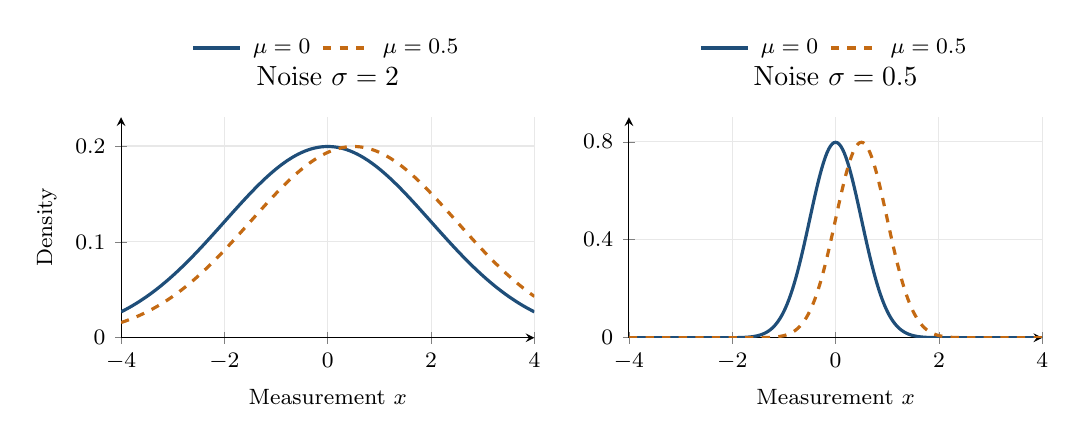
\begin{tikzpicture}
\begin{groupplot}[
  group style={group size=2 by 1,horizontal sep=1.2cm},
  info axis,width=5.25cm,height=2.8cm,
  xmin=-4,xmax=4,xlabel={Measurement $x$},
  xtick={-4,-2,0,2,4},scaled ticks=false,
  title style={font=\normalsize,yshift=2pt},
  legend style={font=\footnotesize,at={(0.5,1.22)},
    anchor=south,legend columns=2,column sep=0.2em},
  domain=-4:4,samples=241]
  \nextgroupplot[title={Noise $\sigma=2$},ymin=0,ymax=0.23,
    ylabel={Density},ytick={0,0.1,0.2}]
  \addplot[InfoBlue] {exp(-x^2/8)/(2*sqrt(2*pi))};
  \addlegendentry{$\mu=0$}
  \addplot[InfoOrange,dashed] {exp(-(x-0.5)^2/8)/(2*sqrt(2*pi))};
  \addlegendentry{$\mu=0.5$}
  \nextgroupplot[title={Noise $\sigma=0.5$},ymin=0,ymax=0.9,
    ytick={0,0.4,0.8}]
  \addplot[InfoBlue] {exp(-x^2/0.5)/(0.5*sqrt(2*pi))};
  \addlegendentry{$\mu=0$}
  \addplot[InfoOrange,dashed] {exp(-(x-0.5)^2/0.5)/(0.5*sqrt(2*pi))};
  \addlegendentry{$\mu=0.5$}
\end{groupplot}
\end{tikzpicture}%
}

\newcommand{\LectureLikelihoodInformationPlot}{%
\begin{tikzpicture}\begin{axis}[info axis,
  width=12cm,height=3.1cm,xmin=-2,xmax=2,ymin=0,ymax=1.04,
  xlabel={Candidate mean minus fitted mean $\mu-\bar x$},
  ylabel={Relative likelihood $L(\mu)/L(\bar x)$},
  xtick={-2,-1,0,1,2},ytick={0,0.25,0.60653066,1},
  yticklabels={$0$,$0.25$,$e^{-1/2}$,$1$}]
  \addplot[InfoOrange] table[x=offset,y=n5] {\InfoDataPath/ch7-likelihood.dat};
  \addlegendentry{$n=5,\ I_n=1.25$}
  \addplot[InfoBlue,dashed] table[x=offset,y=n20] {\InfoDataPath/ch7-likelihood.dat};
  \addlegendentry{$n=20,\ I_n=5$}
  \addplot[InfoTeal] table[x=offset,y=n80] {\InfoDataPath/ch7-likelihood.dat};
  \addlegendentry{$n=80,\ I_n=20$}
  \addplot[InfoMuted,densely dotted,forget plot]
    coordinates {(-2,0.60653066) (2,0.60653066)};
  \addplot[InfoOrange,only marks,mark=*,mark size=2pt,forget plot]
    coordinates {(0.89442719,0.60653066)};
  \addplot[InfoBlue,only marks,mark=*,mark size=2pt,forget plot]
    coordinates {(0.44721360,0.60653066)};
  \addplot[InfoTeal,only marks,mark=*,mark size=2pt,forget plot]
    coordinates {(0.22360680,0.60653066)};
\end{axis}\end{tikzpicture}%
}

\title{Entropy, KL divergence, and Fisher information}
\subtitle{Lecture 7}
\author{}
\date{Scientific Computing 2026}
\hypersetup{pdftitle={Lecture 7: Entropy, KL divergence, and Fisher information},
  pdfsubject={Scientific Computing 2026, Chapter 7},pdfauthor={}}

\begin{document}

% 1
{\setbeamercolor{background canvas}{bg=Ink}
\begin{frame}[plain]
\slidespacing
\color{white}
{\large Scientific Computing 2026\par}
\vfill
{\LARGE\bfseries Entropy, KL divergence,\par
and Fisher information\par}
\vfill
{\large Lecture 7\par}\vspace{4mm}
\end{frame}}

% 2 -- Conspect 7.1
\begin{frame}{A rare outcome carries more surprise}
\slidespacing
Assume a population with two labels:
\[
  \Prob(Y=1)=0.8,\qquad \Prob(Y=0)=0.2.
\]
\begin{definitionbox}{Surprisal}
An outcome of probability \(p>0\) has surprisal \(-\log p\).
We use natural logarithms; the unit is a \emph{nat}.
\end{definitionbox}
\[
  -\log0.8\approx0.2231,\qquad -\log0.2\approx1.6094.
\]
For independent outcomes, surprise adds:
\[
  -\log(p_1p_2)=-\log p_1-\log p_2.
\]
\end{frame}

% 3
\begin{frame}{Entropy averages the surprise}
\slidespacing
Let \(P=(p_1,\ldots,p_K)\) be probabilities for \(K\) labels.
\begin{definitionbox}{Entropy}
\[
  H(P)=\Expect_{Y\sim P}[-\log p_Y]
      =-\sum_{k=1}^{K}p_k\log p_k,
  \qquad 0\log0:=0.
\]
\end{definitionbox}
For the population with \(80\%\) successes,
\[
  H(P)=-0.8\log0.8-0.2\log0.2\approx0.5004.
\]
If one label has probability one, \(H(P)=0\).
\end{frame}

% 4
\begin{frame}{Bernoulli entropy is largest at \(p=1/2\)}
\slidespacing
Write \(P_p=\operatorname{Bernoulli}(p)\):
\[
  H(P_p)=-p\log p-(1-p)\log(1-p).
\]
\centering\InfoEntropyPlot
\plotcaption{A balanced label is hardest to predict.
The maximum is \(\log2\approx0.6931\) nats.}
\end{frame}

% 5 -- Conspect 7.2
\begin{frame}{Evaluate predictions using the actual outcomes}
\slidespacing
\(P=(p_1,\ldots,p_K)\): population probabilities.\par
\(Q=(q_1,\ldots,q_K)\): predicted probabilities for the same labels.
\begin{definitionbox}{Cross-entropy}
\[
  \CE(P,Q)=\Expect_{Y\sim P}[-\log q_Y]
         =-\sum_{k=1}^K p_k\log q_k.
\]
\end{definitionbox}
If the population success probability is \(0.8\), but we predict \(q\),
\[
  \CE(P_{0.8},P_q)=-0.8\log q-0.2\log(1-q).
\]
If \(p_k>0\) but \(q_k=0\), the expected loss is infinite.
\end{frame}

% 6
\begin{frame}{Overconfident errors are expensive}
\slidespacing
Keep the population success probability fixed at \(0.8\).
\par\medskip
{\renewcommand{\arraystretch}{1.5}
\begin{tabular*}{\textwidth}{@{\extracolsep{\fill}}lrr@{}}
\toprule
Predicted \(q\) & Expected log loss & Excess over \(0.5004\)\\
\midrule
\(0.50\) & \(0.6931\) & \(0.1927\)\\
\(0.60\) & \(0.5919\) & \(0.0915\)\\
\(0.80\) & \(0.5004\) & \(0\)\\
\(0.99\) & \(0.9291\) & \(0.4287\)\\
\bottomrule
\end{tabular*}}
\par\medskip
At \(q=0.99\), a failure has loss \(-\log0.01\approx4.6052\).
Failures occur \(20\%\) of the time in this population.
\end{frame}

% 7
\begin{frame}{KL is the extra expected log loss}
\slidespacing
\begin{definitionbox}{Kullback--Leibler divergence}
\[
  \KL(P\Vert Q)=\sum_{k:p_k>0}p_k\log\frac{p_k}{q_k}.
\]
It is infinite if a positive \(p_k\) is paired with \(q_k=0\).
\end{definitionbox}
Subtract the entropy from the cross-entropy:
\[
  -\sum_kp_k\log q_k+\sum_kp_k\log p_k
  =\sum_kp_k\log\frac{p_k}{q_k}.
\]
\begin{resultbox}{Entropy plus mismatch}
\[
  \CE(P,Q)=H(P)+\KL(P\Vert Q).
\]
\end{resultbox}
\end{frame}

% 8
\begin{frame}{Why KL cannot be negative}
\slidespacing
Use the scalar inequality \(-\log u\ge1-u\), with equality only at \(u=1\).
For positive \(p_k\), set \(u=q_k/p_k\):
\[
  \begin{aligned}
  \KL(P\Vert Q)
    &=\sum_{k:p_k>0}p_k\!\left(-\log\frac{q_k}{p_k}\right)\\
    &\ge\sum_{k:p_k>0}(p_k-q_k)\ge0.
  \end{aligned}
\]
\begin{resultbox}{Best prediction for a fixed population}
\(\KL(P\Vert Q)\ge0\), with equality exactly when \(Q=P\).\par
Therefore \(\CE(P,Q)\ge H(P)\).
\end{resultbox}
\end{frame}

% 9
\begin{frame}{The direction of KL changes the answer}
\slidespacing
For \(P=P_{0.8}\) and \(Q=P_{0.5}\),
\[
  \begin{aligned}
  \KL(P\Vert Q)
    &=0.8\log\frac{0.8}{0.5}
      +0.2\log\frac{0.2}{0.5}
      \approx0.1927,\\[0.5em]
  \KL(Q\Vert P)
    &=0.5\log\frac{0.5}{0.8}
      +0.5\log\frac{0.5}{0.2}
      \approx0.2231.
  \end{aligned}
\]
The first distribution supplies the averaging probabilities.
\medskip
KL is not symmetric, so it is not a distance.
\end{frame}

% 10
\begin{frame}{Entropy stays fixed; mismatch changes}
\slidespacing
\centering\InfoCrossEntropyPlot
\plotcaption{Population \(p=0.8\). The vertical gap between cross-entropy
and entropy is KL. The best prediction is \(q=0.8\).}
\end{frame}

% 11 -- Conspect 7.3
\begin{frame}{Maximum likelihood minimizes empirical cross-entropy}
\slidespacing
For \(n\) independent labels, let \(\widehat p_k=n_k/n\), where \(n_k\)
counts label \(k\). The model predicts \(q_\theta(k)\).
\[
  \begin{aligned}
  -\frac1n\log L(\theta)
  &=-\frac1n\sum_{i=1}^n\log q_\theta(y_i)\\
  &=-\sum_{k=1}^K\widehat p_k\log q_\theta(k)
   =\CE(\widehat P,Q_\theta).
  \end{aligned}
\]
\begin{resultbox}{Same minimizer}
\[
  \CE(\widehat P,Q_\theta)
   =\underbrace{H(\widehat P)}_{\text{fixed data}}
     +\KL(\widehat P\Vert Q_\theta).
\]
\end{resultbox}
This empirical KL identity is for finite labels, not continuous densities.
\end{frame}

% 12
\begin{frame}{Multiclass loss selects the observed label}
\slidespacing
For input \(x\), the model predicts \(q_\theta(k\mid x)\).
If the observed label is \(y\), the one-hot target is
\[
  t_k=\begin{cases}1,&k=y,\\0,&k\ne y.\end{cases}
\]
Its cross-entropy is
\[
  -\sum_{k=1}^K t_k\log q_\theta(k\mid x)
  =-\log q_\theta(y\mid x).
\]
Example: \(y=2\) and predicted probabilities \((0.6,0.3,0.1)\):
\[
  \text{loss}=-\log0.3\approx1.2040.
\]
\end{frame}

% 13
\begin{frame}{Language-model loss is conditional log loss}
\slidespacing
For an observed sequence \(w_1,\ldots,w_m\), the chain rule gives
\[
  Q_\theta(w_1,\ldots,w_m)
  =\prod_{t=1}^{m}q_\theta(w_t\mid w_1,\ldots,w_{t-1}).
\]
The condition is empty for \(t=1\). The average token loss is
\[
  -\frac1m\sum_{t=1}^m\log q_\theta(w_t\mid w_1,\ldots,w_{t-1}).
\]
If three observed tokens receive probabilities \(0.5,\ 0.25,\ 0.1\),
\[
  Q_\theta(\text{sequence})=0.0125,\qquad
  \text{average loss}=-\frac{\log0.0125}{3}\approx1.4607.
\]
The tokens do not need to be independent.
\end{frame}

% 14
\begin{frame}{Distillation uses probability targets}
\slidespacing
For the same input, a teacher gives probabilities \(P\);
a student gives probabilities \(Q\):
\[
  P=(0.7,0.2,0.1),\qquad Q=(0.6,0.25,0.15).
\]
Train the student using all teacher probabilities:
\[
  \CE(P,Q)=-0.7\log0.6-0.2\log0.25-0.1\log0.15
  \approx0.8245.
\]
\[
  \underbrace{\CE(P,Q)}_{0.8245}
  =\underbrace{H(P)}_{0.8018}
   +\underbrace{\KL(P\Vert Q)}_{0.0227}.
\]
The teacher entropy is fixed, so minimizing cross-entropy minimizes this KL.
\end{frame}

% 15
\begin{frame}{A KL penalty can keep predictions near a reference}
\slidespacing
For a specified input, let \(Q_\theta\) be the model prediction
and \(Q_{\mathrm{ref}}\) a fixed reference on the same labels.
\[
  \mathcal L_{\mathrm{train}}(\theta)
  +\beta\KL(Q_\theta\Vert Q_{\mathrm{ref}}),
  \qquad \beta\ge0.
\]
\(\mathcal L_{\mathrm{train}}\) is the training loss;
\(\beta\) controls the penalty strength.
\[
  \KL(Q_\theta\Vert Q_{\mathrm{ref}})
  =\sum_k q_\theta(k)\log\frac{q_\theta(k)}{q_{\mathrm{ref}}(k)}.
\]
A reference probability of zero forbids positive model mass there
when \(\beta>0\). This penalty concerns outputs; MAP used a prior on parameters.
\end{frame}

% 16 -- Conspect 7.4
\begin{frame}{Distinguishing two possible means}
\slidespacing
For \(X\sim\mathcal N(\mu,\sigma^2)\), compare \(\mu=0\) with \(\mu=0.5\).
\medskip
\centering\LectureMeanSensitivityPlot
\plotcaption{Both panels use the same horizontal scale and a mean shift of \(0.5\).
Less noise makes the two possible means easier to distinguish from data.}
\end{frame}

% 17
\begin{frame}{The score tells us which way an observation pushes}
\slidespacing
Let \(f_\theta(x)\) be a PMF or density with scalar parameter \(\theta\).
\begin{definitionbox}{Score of one observation}
\[
  s_\theta(x)=\frac{\partial}{\partial\theta}\log f_\theta(x).
\]
\end{definitionbox}
For \(X\sim\mathcal N(\mu,\sigma^2)\), with known \(\sigma^2\),
\[
  s_\mu(x)=\frac{x-\mu}{\sigma^2}.
\]
If \(x>\mu\), increasing \(\mu\) raises this observation's log-likelihood.
If \(x<\mu\), decreasing \(\mu\) raises it.
\end{frame}

% 18
\begin{frame}{Observed information at the fitted maximum}
\slidespacing
For the recorded sample, let \(\ell_n(\theta)=\log L(\theta)\).
Its derivative is the sample score \(S_n(\theta)=\ell_n'(\theta)\).
\[
  S_n(\widehat\theta)=0
  \qquad\text{at a differentiable interior MLE.}
\]
Both a flat peak and a sharp peak have zero slope.
\begin{definitionbox}{Observed information}
\[
  J_n(\theta)=-\ell_n''(\theta).
\]
It describes the downward curvature for this particular dataset.
\end{definitionbox}
At a fitted peak, larger positive \(J_n\) means a sharper peak.
\end{frame}

% 19
\begin{frame}{The likelihood drop near its maximum}
\slidespacing
Let \(\delta\) be a small change from the MLE \(\widehat\theta\).
The zero slope leaves the quadratic term:
\[
  \ell_n(\widehat\theta+\delta)-\ell_n(\widehat\theta)
     \approx-\frac12 J_n(\widehat\theta)\delta^2.
\]
For the same change \(\delta=0.1\):
\par\medskip
{\renewcommand{\arraystretch}{1.5}
\begin{tabular*}{\textwidth}{@{\extracolsep{\fill}}lrr@{}}
\toprule
Curvature \(J_n(\widehat\theta)\) & Log-likelihood change & Likelihood ratio\\
\midrule
\(4\) & \(-0.02\) & \(e^{-0.02}\approx0.980\)\\
\(100\) & \(-0.5\) & \(e^{-0.5}\approx0.607\)\\
\bottomrule
\end{tabular*}}
\par\medskip
The ratio compares \(L(\widehat\theta+0.1)\) with \(L(\widehat\theta)\).
The larger curvature gives a larger drop.
\end{frame}

% 20
\begin{frame}{Fisher information averages over possible datasets}
\slidespacing
Keep \(\theta\) fixed. Draw new datasets from that model and calculate
their curvatures at the same \(\theta\).
\begin{definitionbox}{Fisher information}
For a regular model,
\[
  I_n(\theta)=\Expect_\theta[J_n(\theta)].
\]
For one observation,
\[
  I_1(\theta)=-\Expect_\theta[
     \partial_\theta^2\log f_\theta(X)].
\]
\end{definitionbox}
\(J_n\) depends on the observed sample.
\(I_n\) averages over possible samples, without refitting \(\theta\) each time.
\end{frame}

% 21
\begin{frame}{Why the score has mean zero}
\slidespacing
Assume common support, an interior parameter, and differentiability
allowing derivatives through the sum or integral.
\[
  \begin{aligned}
  \Expect_\theta[s_\theta(X)]
  &=\int \frac{\partial_\theta f_\theta(x)}{f_\theta(x)}
             f_\theta(x)\,dx\\
  &=\frac{\partial}{\partial\theta}\int f_\theta(x)\,dx
    =\frac{\partial}{\partial\theta}1=0.
  \end{aligned}
\]
For a discrete law, replace the integral by a sum.
\medskip
For the Gaussian mean: \(\Expect_\mu[(X-\mu)/\sigma^2]=0\).
\end{frame}

% 22
\begin{frame}{Fisher information as an expected squared score}
\slidespacing
Differentiate the log-likelihood twice:
\[
  \partial_\theta^2\log f_\theta
  =\frac{\partial_\theta^2 f_\theta}{f_\theta}
   -\left(\frac{\partial_\theta f_\theta}{f_\theta}\right)^2.
\]
The first term has expectation
\(\int\partial_\theta^2 f_\theta(x)\,dx=\partial_\theta^2 1=0\).
\begin{resultbox}{Equivalent score formula}
With a finite score second moment,
\[
  I_1(\theta)=\Expect_\theta[s_\theta(X)^2]
            =\Var_\theta(s_\theta(X)).
\]
\end{resultbox}
The fitted sample score is zero. Scores on new datasets at a fixed
parameter vary, so their expected square need not be zero.
\end{frame}

% 23
\begin{frame}{Gaussian noise and information about the mean}
\slidespacing
For the Gaussian mean with known variance,
\[
  I_1(\mu)
  =\frac{\Expect_\mu[(X-\mu)^2]}{\sigma^4}
  =\frac1{\sigma^2}.
\]
\par\medskip
{\renewcommand{\arraystretch}{1.5}
\begin{tabular*}{\textwidth}{@{\extracolsep{\fill}}lrr@{}}
\toprule
Observation noise & \(\sigma\) & Information \(I_1(\mu)\)\\
\midrule
More noise & \(2\) & \(0.25\)\\
Less noise & \(0.5\) & \(4\)\\
\bottomrule
\end{tabular*}}
\par\medskip
These are the two noise levels in the earlier density plots.
The smaller noise gives sixteen times as much information about \(\mu\).
\end{frame}

% 24
\begin{frame}{Independent observations add information}
\slidespacing
For \(n\) i.i.d. observations,
\[
  \ell_n(\theta)=\sum_{i=1}^n\log f_\theta(X_i),\qquad
  S_n(\theta)=\ell_n'(\theta)=\sum_{i=1}^n s_\theta(X_i).
\]
Independence and zero mean scores give
\[
  I_n(\theta)=\Var_\theta(S_n(\theta))
   =\sum_{i=1}^n\Var_\theta(s_\theta(X_i))
   =nI_1(\theta).
\]
For Gaussian measurements with known variance \(\sigma^2\),
\[
  I_n(\mu)=\frac n{\sigma^2}.
\]
\end{frame}

% 25
\begin{frame}{Gaussian mean: observed and expected information}
\slidespacing
For \(n\) independent measurements with known variance \(\sigma^2\),
\[
  \ell_n(\mu)=C-\frac{n}{2\sigma^2}(\mu-\bar x)^2,
\]
where \(C\) does not depend on the candidate mean \(\mu\).
\[
  J_n(\mu)=-\ell_n''(\mu)=\frac{n}{\sigma^2}=I_n(\mu).
\]
\begin{resultbox}{The same curvature for every possible dataset}
\[
  \frac{L(\mu)}{L(\bar x)}
     =\exp\!\left[-\frac12 I_n(\mu)(\mu-\bar x)^2\right].
\]
\end{resultbox}
\end{frame}

% 26
\begin{frame}{Larger information gives a narrower likelihood peak}
\slidespacing
Known \(\sigma=2\), so \(J_n=I_n=n/4\).
At a distance \(1/\sqrt{I_n}\) from the peak, relative likelihood is \(e^{-1/2}\).
\medskip
\centering\LectureLikelihoodInformationPlot
\plotcaption{Marked distances: \(0.894,\ 0.447,\ 0.224\).
Larger \(I_n\) gives a narrower peak.}
\end{frame}

% 27
\begin{frame}{Bernoulli score: successes and failures pull differently}
\slidespacing
Now the success probability \(p\in(0,1)\) is unknown.
For \(Y\sim\operatorname{Bernoulli}(p)\),
\[
  \log f_p(y)=y\log p+(1-y)\log(1-p),
\]
\[
  s_p(y)=\frac y p-\frac{1-y}{1-p}
        =\frac{y-p}{p(1-p)}.
\]
At \(p=0.8\),
\[
  s_p(1)=1.25,\qquad s_p(0)=-5,\qquad
  0.8(1.25)+0.2(-5)=0.
\]
A rare failure gives a larger push toward lowering \(p\).
\end{frame}

% 28
\begin{frame}{Bernoulli Fisher information}
\slidespacing
Use \(\Var(Y)=p(1-p)\):
\[
  \begin{aligned}
  I_1(p)
   &=\Expect_p\!\left[\frac{(Y-p)^2}{p^2(1-p)^2}\right]\\
   &=\frac{p(1-p)}{p^2(1-p)^2}
    =\frac1{p(1-p)}.
  \end{aligned}
\]
\begin{resultbox}{A sample of independent labels}
\[
  I_n(p)=\frac n{p(1-p)}.
\]
At \(p=0.8\), one label gives \(I_1=6.25\);
\(100\) labels give \(I_{100}=625\).
\end{resultbox}
\end{frame}

% 29
\begin{frame}{Observed and expected information can differ}
\slidespacing
For \(10\) Bernoulli trials, let \(k\) be the observed success count:
\[
  J_{10}(p)=\frac{k}{p^2}+\frac{10-k}{(1-p)^2}.
\]
Evaluate different datasets at the same fixed \(p=0.8\):
\par\medskip
{\renewcommand{\arraystretch}{1.5}
\begin{tabular*}{\textwidth}{@{\extracolsep{\fill}}lrr@{}}
\toprule
Successes \(k\) & Observed \(J_{10}(0.8)\) & Expected \(I_{10}(0.8)\)\\
\midrule
\(7\) & \(85.94\) & \(62.5\)\\
\(9\) & \(39.06\) & \(62.5\)\\
\bottomrule
\end{tabular*}}
\par\medskip
Fisher information averages over all possible success counts,
using their probabilities under \(p=0.8\).
\end{frame}

% 30
\begin{frame}{Bernoulli entropy and information}
\slidespacing
\centering\InfoFisherPlot
\plotcaption{Entropy is largest at \(p=1/2\); information about \(p\)
is smallest there. The sample proportion's absolute variance,
\(p(1-p)/n\), is also largest at \(p=1/2\).}
\end{frame}

% 31 -- Conspect 7.5
\begin{frame}{How small can an unbiased estimator's variance be?}
\slidespacing
\begin{resultbox}{Cramér--Rao lower bound}
For a regular model, let \(T\) estimate the scalar parameter \(\theta\).
If \(T\) has finite variance, is unbiased throughout an open parameter
interval, and differentiation of its expectation is valid, then
\[
  \Var_\theta(T)\ge\frac1{I_n(\theta)}
                 =\frac1{nI_1(\theta)},\qquad
  0<I_n(\theta)<\infty.
\]
\end{resultbox}
\begin{definitionbox}{Efficient unbiased estimator}
An unbiased estimator attaining this bound is efficient
at that parameter value.
\end{definitionbox}
\end{frame}

% 32
\begin{frame}{Cramér--Rao proof: differentiating unbiasedness}
\slidespacing
Write \(x=(x_1,\ldots,x_n)\), and let \(g_\theta(x)\) be the joint sample density.
The rule \(T(x)\) does not use the unknown \(\theta\).
\[
  \begin{aligned}
  \Expect_\theta T=\theta
  &\quad\Longrightarrow\quad
  1=\frac{\partial}{\partial\theta}\int T(x)g_\theta(x)\,dx\\
  &=\int T(x)\,\partial_\theta g_\theta(x)\,dx.
  \end{aligned}
\]
Use \(\partial_\theta g_\theta=g_\theta\,\partial_\theta\log g_\theta\).
The log-derivative is the sample score \(S_n(\theta)\), hence
\[
  1=\int T(x)g_\theta(x)\,\partial_\theta\log g_\theta(x)\,dx
    =\Expect_\theta[T S_n(\theta)].
\]
For a discrete sample, use sums instead of integrals.
\end{frame}

% 33
\begin{frame}{Cramér--Rao proof: the covariance bound}
\slidespacing
The previous step gave \(\Expect_\theta[T S_n(\theta)]=1\).
Since \(\Expect_\theta S_n(\theta)=0\),
\[
  \begin{aligned}
  \Cov_\theta(T,S_n(\theta))
   &=\Expect_\theta[T S_n(\theta)]
       -\Expect_\theta T\,\Expect_\theta S_n(\theta)\\
   &=1-\theta\cdot0=1.
  \end{aligned}
\]
Lecture 3's inequality \(\Cov(U,V)^2\le\Var(U)\Var(V)\) now gives
\[
  1\le\Var_\theta(T)\underbrace{\Var_\theta(S_n(\theta))}_{I_n(\theta)}.
\]
Divide by \(I_n(\theta)>0\):
\(\displaystyle\Var_\theta(T)\ge1/I_n(\theta)\).
\end{frame}

% 34
\begin{frame}{The Gaussian sample mean attains the bound}
\slidespacing
For \(X_i\sim\mathcal N(\mu,\sigma^2)\) independently,
with known \(\sigma^2\),
\[
  I_n(\mu)=\frac n{\sigma^2},\qquad
  \Var_\mu(\bar X_n)=\frac{\sigma^2}n=\frac1{I_n(\mu)}.
\]
The sample mean is unbiased and efficient.
\par\medskip
{\renewcommand{\arraystretch}{1.5}
\begin{tabular*}{\textwidth}{@{\extracolsep{\fill}}lll@{}}
\toprule
Estimator & Expectation & Variance\\
\midrule
\(\bar X_n\) & \(\mu\) & \(\sigma^2/n\)\\
\(X_1\) & \(\mu\) & \(\sigma^2\)\\
\bottomrule
\end{tabular*}}
\par\medskip
Using only the first measurement is unbiased but discards data.
\end{frame}

% 35
\begin{frame}{The sample mean follows the information bound}
\slidespacing
\centering\InfoVariancePlot
\plotcaption{\(X_i\sim\mathcal N(\mu,4)\) independently.
The points use \(30{,}000\) simulated datasets per \(n\).
The first-observation estimator has variance \(4\) at every \(n\).}
\end{frame}

% 36
\begin{frame}{The Bernoulli sample proportion is also efficient}
\slidespacing
For \(n\) independent Bernoulli labels, with \(0<p<1\),
\[
  \widehat p=\frac1n\sum_{i=1}^nY_i,\qquad
  \Expect_p\widehat p=p.
\]
\[
  \Var_p(\widehat p)=\frac{p(1-p)}n
     =\frac1{I_n(p)}.
\]
At \(p=0.8,\ n=100\),
\[
  \Var_p(\widehat p)=0.0016,\qquad
  \operatorname{SE}_p(\widehat p)=0.04.
\]
This variance is exact. A Gaussian approximation to the sampling
distribution is still an approximation.
\end{frame}

% 37
\begin{frame}{A biased estimator can have smaller variance}
\slidespacing
For the Gaussian mean, consider \(T=\bar X_n/2\):
\[
  \Var_\mu(T)=\frac{\sigma^2}{4n}
     <\underbrace{\frac{\sigma^2}n}_{\text{unbiased variance bound}},
  \qquad
  \Expect_\mu T-\mu=-\frac\mu2.
\]
Its mean squared error includes both terms:
\[
  \Expect_\mu[(T-\mu)^2]
   =\frac{\sigma^2}{4n}+\frac{\mu^2}{4}.
\]
The Cramér--Rao statement above requires unbiasedness.
\end{frame}

% 38 -- Conspect 7.6
\begin{frame}{A Gaussian approximation for an MLE}
\slidespacing
The Bernoulli MLE is a sample average, so its Gaussian approximation
comes from the CLT. Regular MLEs have a similar large-sample behavior.
\begin{resultbox}{Approximate sampling distribution}
For true parameter \(\theta\) and MLE \(\widehat\theta\),
\[
  \widehat\theta\ \text{is approximately}\ %
  \mathcal N\!\left(\theta,\frac1{I_n(\theta)}\right).
\]
\end{resultbox}
This requires a consistent MLE away from parameter boundaries
and regular likelihood behavior near the true value.
It gives no finite-sample unbiasedness guarantee.
\end{frame}

% 39
\begin{frame}{Estimating the error scale from eighty successes}
\slidespacing
The probability \(p\) is unknown. Observing \(80\) successes in \(100\)
independent trials gives \(\widehat p=0.8\).
\[
  I_{100}(p)=\frac{100}{p(1-p)}
  \qquad\text{so}\qquad
  I_{100}(\widehat p)=\frac{100}{0.8(0.2)}=625.
\]
\begin{resultbox}{Estimated standard error}
\[
  \widehat{\operatorname{SE}}(\widehat p)
   =\frac1{\sqrt{I_{100}(\widehat p)}}
   =\frac1{\sqrt{625}}=0.04.
\]
\end{resultbox}
We substitute the fitted probability for the unknown \(p\)
to estimate the sampling spread.
\end{frame}

% 40
\begin{frame}{The corresponding confidence interval}
\slidespacing
For the same \(100\) trials, \(\widehat p=0.8\) and
\(\widehat{\operatorname{SE}}=0.04\).
\begin{resultbox}{Approximate \(95\%\) confidence interval}
\[
  \widehat p\pm1.96\,\widehat{\operatorname{SE}}
  =0.8\pm0.0784
  =[0.7216,\ 0.8784].
\]
\end{resultbox}
This is the Wald interval from Lecture 6.
Fisher information gives its error scale.
\medskip
The Gaussian approximation can still be poor near \(p=0\) or \(p=1\),
especially with few observations.
\end{frame}

% 41 -- Conspect 7.7
\begin{frame}{Nearby distributions and Fisher information}
\slidespacing
Let \(P_\theta\) be a regular model and let \(\delta\) be a small
change in its parameter.
\begin{resultbox}{KL for a small parameter change}
\[
  \KL(P_\theta\Vert P_{\theta+\delta})
    \approx\frac12 I_1(\theta)\delta^2.
\]
\end{resultbox}
KL is zero when the two parameter values coincide.
Fisher information sets how quickly it grows for small changes.
\medskip
For Bernoulli \(p=0.8\), \(I_1(p)=6.25\), giving
\[
  \KL(P_{0.8}\Vert P_{0.8+\delta})\approx3.125\,\delta^2.
\]
\end{frame}

% 42
\begin{frame}{Bernoulli KL near \(p=0.8\)}
\slidespacing
\renewcommand{\InfoPlotHeight}{3.15cm}
Quadratic approximation:
\(\tfrac12 I_1(0.8)(q-0.8)^2=3.125(q-0.8)^2\).
\medskip
\centering\InfoLocalKLPlot
\plotcaption{Here \(\delta=q-0.8\).
The quadratic curve agrees near \(q=0.8\), then loses accuracy farther away.}
\end{frame}

\end{document}
